\documentclass{article}
\usepackage[T1]{fontenc}
\usepackage{lmodern}
\usepackage{graphicx}
\usepackage{amsmath,amssymb}
\usepackage[a4paper,margin=2cm]{geometry}
\usepackage[absolute,overlay]{textpos}
\setlength{\TPHorizModule}{1mm}
\setlength{\TPVertModule}{1mm}
\usepackage[indonesian]{babel}
\usepackage{hyperref}
\setlength{\emergencystretch}{2em}
% unit: Halaman 9

\begin{document}

% === Halaman 9 (llm) ===

\section*{Operasi XOR}

\begin{itemize}
    \item Di dalam \textit{cipher} modern, operasi XOR adalah operasi yang paling sering digunakan
    \item Notasi: $\oplus$
    \item Operasi:
    \[
    \begin{aligned}
    0 \oplus 0 &= 0 & 0 \oplus 1 &= 1 \\
    1 \oplus 0 &= 1 & 1 \oplus 1 &= 0
    \end{aligned}
    \]
\end{itemize}

\vspace{10mm}

% deskripsi: Tabel kebenaran untuk operasi XOR dengan kolom a, b, dan hasil a XOR b.
% bbox normalisasi: [0.1920, 0.6280, 0.4380, 0.9150]
\begin{textblock*}{51.66mm}(40.32mm,186.52mm)
\noindent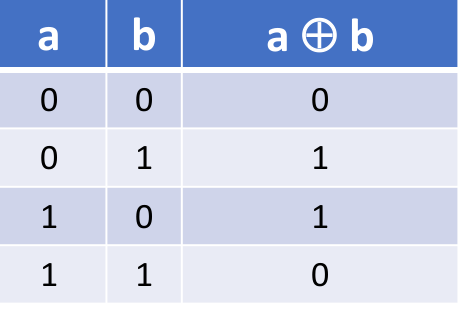
\includegraphics[width=51.66mm,height=85.24mm]{../../images/llm/page_009_img_01.png}%
\end{textblock*}

\end{document}
